\documentclass[tikz,border=12pt]{standalone}
\usepackage{amsmath,amssymb}
\usetikzlibrary{calc,arrows.meta}

\begin{document}
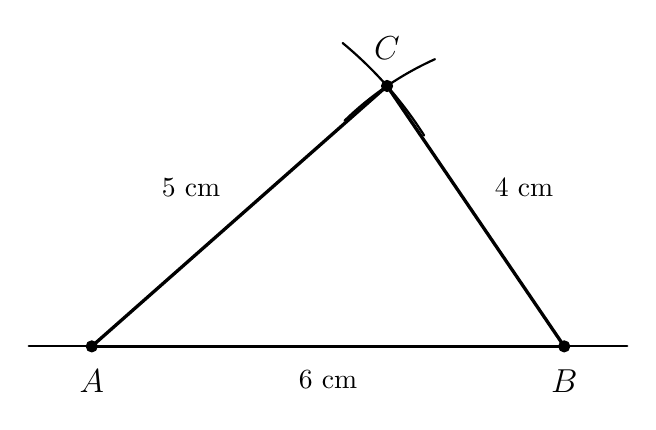
\begin{tikzpicture}[>=latex, line cap=round, line join=round]
  % Side lengths: c = 6.0, b = 5.0, a = 4.0
  \def\c{6.0}
  \def\b{5.0}
  \def\a{4.0}

  % Coordinates
  \coordinate (A) at (0, 0);
  \coordinate (B) at (\c, 0);

  % Apex C: x = 3.75, y = sqrt(25 - 3.75^2) = 3.307
  \pgfmathsetmacro{\xC}{(\b*\b - \a*\a + \c*\c) / (2*\c)}
  \pgfmathsetmacro{\yC}{sqrt(\b*\b - \xC*\xC)}
  \coordinate (C) at (\xC, \yC);

  % Baseline extension
  \draw[thick] (-0.8, 0) -- ({\c + 0.8}, 0);

  % Triangle ABC
  \draw[very thick] (A) -- (B) node[midway, below=5pt, font=\normalsize] {$6\text{ cm}$};
  \draw[very thick] (A) -- (C) node[midway, above left=3pt, font=\normalsize] {$5\text{ cm}$};
  \draw[very thick] (B) -- (C) node[midway, above right=3pt, font=\normalsize] {$4\text{ cm}$};

  % Vertices
  \filldraw[black] (A) circle (2pt) node[below=5pt, font=\large\bfseries] {$A$};
  \filldraw[black] (B) circle (2pt) node[below=5pt, font=\large\bfseries] {$B$};
  \filldraw[black] (C) circle (2pt) node[above=6pt, font=\large\bfseries] {$C$};

  % Construction arc from A (radius b) through C
  \pgfmathsetmacro{\angA}{atan2(\yC, \xC)}
  \draw[thick] ($(A) + ({\angA - 9}:\b)$) arc ({\angA - 9}:{\angA + 9}:\b);

  % Construction arc from B (radius a) through C
  \pgfmathsetmacro{\angB}{atan2(\yC, \xC - \c)}
  \draw[thick] ($(B) + ({\angB - 10}:\a)$) arc ({\angB - 10}:{\angB + 10}:\a);

\end{tikzpicture}
\end{document}
